\subsection*{A. A sad number}

Ввиду некоторых печальных событий, никак не связанных с учёбой в университете, Денис считает цифру 2 самой грустной цифрой. Соответственно натуральные числа, в десятичной записи которых есть цифра 2, Денис называет <<грустными>> числами; числам же, которые можно разложить на сумму двух <<грустных>> чисел, Денис дал название <<очень грустные>> числа. Поскольку определение вышло слишком сложным, помогите Денису определить, является ли данное число <<очень грустным>> или нет.

\informat{Одно целое число $n$, где $1 \le n \le 10^{18}$.}

\outformat{Слово YES, если введенное число является <<очень грустным>>, и NO --- иначе.}

\exampleee{10}{NO}{14}{YES}{3018}{YES}

\excomm{Число 10 нельзя разложить на сумму двух грустных чисел. \newline
Число 14 = 12 + 2, здесь и 2, и 12 содержат двойку в своей записи. \newline
Число 3018 = 2016 + 1002 --- оба слагаемых являются грустными числами.}



\subsection*{B. Brute force}

Тимур считает, что все задачи по программированию можно решить перебором. Казалось бы, чего сложного, например, перебрать все возможные пары различных натуральных чисел $(a, b)$ не более некоторого $n$ и вывести максимальный НОД из полученных? Не правда ли?

\informat{Одно целое число $n$, где $2 \le n \le 10^{18}$.}

\outformat{Одно целое число --- максимальный НОД чисел $a$ и $b$ при всех возможных \mbox{$1 \le a < b \le n$.}}

\examplee{2}{1}{5}{2}

\excomm{Во втором примере все возможны НОДы равны: \newline
НОД(1, 2) = 1, НОД(1, 3) = 1, НОД(1, 4) = 1, НОД(1, 5) = 1, НОД(2, 3) = 1, НОД(2, 4) = 2, НОД(2, 5) = 1, НОД(3, 4) = 1, НОД(3, 5) = 1, НОД(4, 5) = 1. \newline
Максимальным из полученных чисел является 2.}



\subsection*{C. Curtains}

Адиль хочет применить полученные знания на практике после окончания университета. Чтобы стать ближе к проектированию <<умного дома>>, Адиль уже сейчас пытается написать что-то своё. Его первый проект --- автоматическое управление шторами. Деталей разработки своего проекта Адиль не раскрывает, но на данный момент его у него имеется $N$ петелек для штор, которые крепятся к карнизу в точках $a_1$, $a_2$, ... , $a_N$ (координаты в см \mbox{$1 \le a_1 < a_2 < \dots < a_N \le 10^5$}). А его <<умный дом>> может выполнять запросы вида:
\begin{enumerate}
\item сдвинуть k-ю петельку вправо или влево на 1 см;
\item сдвинуть k-ю петельку вправо или влево на 1 см.
\end{enumerate}
При этом совпадать петельки в процессе действий не могут --- такие действия следует игнорировать. Проект ещё далёк от завершения, а Адилю нужно готовиться к сессии. Чтобы контролировать, насколько сильно провисают шторы, Адилю важно знать максимальное расстояние между соседними петельками после каждого запроса. Обратите внимание, что карниз можно считать бесконечным и координаты могут становится отрицательными в процессе перемещений.

\informat{В первой строке целое число $N$ --- число штор, где $2 \le N \le 10^5$, \newline
во второй строке $N$ целых чисел $a_1, a_2, \dots, a_N$ --- начальное положение штор, где $1 \le a_i \le 10^5$, \newline
в третьей строке целое число $Q$ --- число запросов, где $1 \le Q \le 10^5$, \newline
в следующих $Q$ строках содержится описания запросов одного из двух видов: \newline
<<R k>> соответствует запросу типа <<сдвинуть k-ую петельку вправо на 1 см>>; \newline
<<L k>> соответствует запросу типа <<сдвинуть k-ую петельку влево на 1 см>>.}

\outformat{$Q$ целых чисел в столбик --- максимальное расстояние между соседними шторами после каждого запроса.}

\examplee{
3 \newline
1 5 10 \newline
3 \newline
R 2 \newline
L 3 \newline
R 1
}
{
5 \newline 5 \newline 4
}
{
2 \newline
1 2 \newline 
3 \newline
R 1 \newline
L 2 \newline
R 2 \newline
}{
1 \newline 1 \newline 2
}



\subsection*{D. Dimitriy and broken sum}

Димитрий отлично знает, как находить сумму членов арифметической прогрессии, поэтому на этот раз ему дали задачку сложнее.
Необходимо найти сумму $a_0 + a_1 + a_2 + ... + a_n$, где $a_i$ отличается от $i$ только $k$-ым битом справа в своей двоичной записи. Если число содержит недостаточно двоичных цифр, следует добавить незначащие нули слева.

\informat{Два целых числа $n$ и $k$, где $0 \le n \le 10^9$ и $1 \le k \le 30$.}

\outformat{Одно целое число --- ответ на задачу.}

\examplee{7 3}{28}{5 3}{23}

\excomm{При $k = 3$ последовательность $\{a_n\}$ будет выглядеть следующим образом: \newline
4, 5, 6, 7, 0, 1, 2, 3, 12, 13, 14, ...}



\subsection*{E. Excursion}

Ребята из команды Snowy Cube сейчас учатся на 3 курсе ВМК и проходят один из самых интересных предметов --- “Машинная графика”, где они программируют отрисовку трёхмерных изображений с помощью библиотеки OpenGL. Как и полагается, первой демонстрационной программой является отрисовка куба. Ребята так хотят научиться писать движки для трехмерных игр, что уже начали разрабатывать трехмерную игру <<Экскурсия по снежному кубу>>. Изначально игровое пространство состоит из куба размера $A$, ребра которого параллельны осям координат. Суть игры заключается в том, чтобы добраться из угла куба $(0, 0, 0)$ в противоположный угол с координатами $(A, A, A)$. Двигаться можно только прыжками по снежинкам, расставленным внутри куба, при этом общая длина всех прыжков не должна превышать данного параметра $K$ (уровень сложности игры). Штраф в игре вычисляется как длина максимального прыжка, совершенного во время преодоления пути. Ясно, что игроки будут пытаться получить минимальный штраф. Чему будет равен абсолютный рекорд для данной карты? 

\informat{В первой строке два целых числа $A$ и $K$ --- размер куба и уровень сложности ($1 \le A \le 1000$, $1 \le K \le 2000$); \newline
во второй строке --- число снежинок $N$ на данной карте ($0 \le N \le 100$); \newline
каждая из следующих $N$ строк содержит три целых числа $x_i$, $y_i$, $z_i$ --- координаты $i$-ой снежинки ($0 \le x_i, y_i, z_i \le A$).}

\outformat{Одно вещественное число --- минимальный штраф $L$ (с точностью в 2 знака после запятой), с которым можно пройти данную карту. Если эту карту на данном уровне сложности пройти невозможно, то вывести -1.}

\exampleeee{
10 20 \newline
5 \newline
5 0 0 \newline
10 0 0 \newline
10 5 0 \newline
10 10 0 \newline
10 10 5}
{17.320}
{10 30 \newline
5 \newline
5 0 0 \newline
10 0 0 \newline
10 5 0 \newline
10 10 0 \newline
10 10 5}
{7.071}
{10 40 \newline
5 \newline
5 0 0 \newline
10 0 0 \newline
10 5 0 \newline
10 10 0 \newline
10 10 5}
{5.000}
{10 16 \newline
2 \newline
6 2 1 \newline
4 0 6}
{-1}



\subsection*{F. Food getting ways}

Знаете ли вы, где можно вкусно перекусить рядом с филиалом МГУ? В соседнем с нашим архитектурно\--строительном корпусе работает замечательная столовая с оригинальным названием The Stolovka. От нашего корпуса до корпуса, в котором находится The Stolovka, можно пройти по одной из двух параллельных аллей, соединённых между собой некоторой системой из попарно не пересекающихся переулков. Ерулан, как большой любитель покушать, собрался посетить данное место. Но, кроме прочего, он еще и большой любитель математики, поэтому он решил воспользоваться случаем и на основе этого маленького приключения составить задачу. 


\begin{center}
\newcommand{\drawblack}[4]{
\draw[line width=20, color=black]
(#1, #2) -- (#3, #4);
}
\newcommand{\drawwhite}[4]{
\draw[line width=18, color=white] 
(#1, #2) -- (#3, #4);
}

\def\picwidth{0.9\linewidth}
\resizebox{\picwidth}{!}{
\begin{tikzpicture}
\drawblack{0}{7}{20}{7}
\drawblack{0}{3}{20}{3}

\drawblack{2}{7}{5}{3}
\drawblack{5}{7}{8}{3}
\drawblack{8}{7}{11}{3}
\drawblack{11}{3}{14}{7}
\drawblack{14}{7}{17}{3}

\drawwhite{-1}{7}{21}{7}
\drawwhite{-1}{3}{21}{3}

\drawwhite{2}{7}{5}{3}
\drawwhite{5}{7}{8}{3}
\drawwhite{8}{7}{11}{3}
\drawwhite{11}{3}{14}{7}
\drawwhite{14}{7}{17}{3}

\node (1) at (0, 7){МГУ};
\node (2) at (20, 3){ЕДА};

\end{tikzpicture}
}
\end{center}

Ерулан записал её условие в следующем формальном виде: две аллеи --- горизонтальные отрезки. Выходит он из верхнего левого угла, прийти должен в правый нижний. Переулки между аллеями бывают 2 видов: {\tt /} и {\tt \textbackslash}. Ерулан всегда движется слева направо. На каждом шаге он может либо продолжить движение по той же аллее, либо перейти по переулку на другую, если есть такая возможность. Посчитайте количество способов попасть в столовую.

\informat{Одно целое число $N$, где $1 \le N \le 10000$. \\
На следующей строке строка длины $N$ из символов вида  '{\tt /}' и '{\tt \textbackslash}'.}

\outformat{Одно целое число --- ответ по модулю $10^9+7$.}

\examplee{
5 \newline
\textbackslash\textbackslash\textbackslash/\textbackslash}
{7}
{2 \newline
//}
{0}

\excomm{обратите внимание, что в языке $C$ и $C$++ константы прямого и обратного слеша обозначаются как {\tt '/'} и {\tt '\textbackslash\textbackslash'}.}



\subsection*{G. Great and Mighty}

Илья учится уже на 4 курсе, но всё ещё отлично помнит что, студенты ВМК за первые три семестра знакомятся с тремя не самыми популярными, но одними из самых важных для понимания основ, языками программирования: pascal, nasm и C. Правда, эта информация никак не помогла ему во время сдачи уравнений математической физики, и навряд ли поможет вам.

\informat{Одно целое число от 1 до 10.}

\examplee{9}{6 5 4}{2}{3 3 3}



\subsection*{H. Hobby}

Темирхан очень обрадовался не столько победе на личной олимпиаде в прошлом году (которая проводится традиционно в декабре в филиале МГУ), сколько подарку в виде сборной модели здания МГУ. Он увлекся различным конструированием, и в частности, задумался о сборке железной дороги. Для этого Темирхан купил себе большую пачку деталей двух видов: прямой прогон (длины 2) или поворот на 90 (ширина 1, высота 1). 

\begin{center}
\def\picwidth{0.45\linewidth}
\resizebox{\picwidth}{!}{
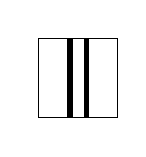
\begin{tikzpicture}
\draw[color=white, rounded corners=10, line width=8] 
(0.5, 0.0) -- (0.5, 0.5) -- (0.0, 0.5);
\draw (0, 0) -- (1, 0) -- (1, 1) -- (0, 1) -- cycle;
\draw[line width=8] 
(0.5, 0.0) -- (0.5, 1.0);
\draw[color=white, line width=4] 
(0.5, 0.0) -- (0.5, 1.0);
\end{tikzpicture}
}
\resizebox{\picwidth}{!}{
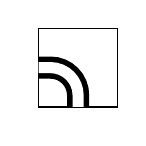
\begin{tikzpicture}
\draw (0, 0) -- (1, 0) -- (1, 1) -- (0, 1) -- cycle;
\draw[rounded corners=10, line width=8] 
(0.5, 0.0) -- (0.5, 0.5) -- (0.0, 0.5);
\draw[color=white, rounded corners=10, line width=4] 
(0.5, 0.0) -- (0.5, 0.5) -- (0.0, 0.5);
\end{tikzpicture}
}
\end{center}

После того, как он принес $A$ деталей первого вида и $B$ деталей второго вида, у него моментально возник вопрос: можно ли составить замкнутую железную дорогу, используя все детали? Помогите ему ответить на этот странный вопрос.

\informat{Два целых числа $A$ и $B$, где $0 \le A \le 10^9$, $0 \le B \le 10^9$ и $A + B > 0$.}

\outformat{Слово YES, если собрать дорогу возможно, и NO --- иначе.}

\exampleee{0 4}{YES}{0 8}{NO}{3 3}{NO}

\excomm{Дорога не может перекрываться, поэтому 8 уголков не подходят.}


\subsection*{I. IMC problem}

Надира и Саша этим летом участвовали в IMC --- международной студенческой олимпиаде по математике в Болгарии. На тренировках они решили огромное количество различных задач, в том числе и по теории чисел. Иногда попадались задачи, которые проще запрограммировать, чем решить честно. Например, как вам такая задача:\newline
\textit{найти $n$-ое число вида $2^p \cdot 5^q$, то есть, $n$-ое число последовательности 1, 2, 4, 5, 8, 10, 16, 20, 25, ...}

\informat{Одно положительное целое число $n$ такое, что ответ гарантированно не превосходит $10^{18}$.}

\outformat{Одно целое число --- $n$-ое число последовательности.}

\exampleee{8}{20}{100}{1000000}{500}{100000000000000}

\newpage

\subsection*{J. Join the knowledge}

Куат изучает очень много математики. За первые два семестра он прослушал курсы <<Алгебра>>, <<Аналитическая геометрия>>, <<Линейная алгебра>> и <<Математический анализ>>. Знания по всем этим предметам занимают большую часть его памяти. Свою память он представляет в виде таблицы $n \times n$. Если клетка памяти занята знаниями, то в таблице это отмечено точкой. Если она еще свободна --- звездочкой. Будучи настоящим математиком, Куат верит, что все предметы и знания по ним должны быть связаны друг с другом (две единицы знаний считаются соседними, если они имеют общую сторону; все единицы считаются связанными между собой, если для любых двух единиц знания $A$ и $B$ можно составить цепочку $A = v_1 \rightarrow v_2 \rightarrow \dots \rightarrow v_k = B$, где $v_i$ и $v_{i+1}$ --- соседние клетки для любого $i$). Куат очень надеется, что его знания связаны друг с другом. А если нет, то он готов потратить еще один вечер и заполнить знаниям еще один кусок памяти, чтобы они стали связаны. Гарантируется, что у Куата уже есть как минимум две единицы знаний. Сможет ли он добиться того, чтобы все его знания стали связаны после добавления одной единицы знаний?

\informat{В первой строке одно целое число $n$, где $2 \le N \le 300$, --- размер матрицы знаний. \newline
На следующих $n$ строках описание таблицы знаний $n \times n$ из символов {\tt *} (звездочка) и {\tt .} (точка).}

\outformat{Слово YES, если Куат может добиться связности знаний, заменив не более одной звездочки на точку, и NO --- иначе.}

\exampleee
{3 \newline
*** \newline
.*. \newline
.*.
}{YES}
{3 \newline
*.* \newline
.*. \newline
*.*
}{YES}
{3 \newline
.*. \newline
*.* \newline
.*.
}{NO}



\subsection*{K. Keg and dipper}

В Казахстанском филиале МГУ с недавнего времени появилась традиция пить чай на тренировках по программированию. Команда Big dipper сразу начала навязывать свои привычки: всё мерить в ковшах, а чай пить только из бесконечно большого бочонка. Ещё ребята определили комфортную температуру чая, при которой его можно пить: от $A$ до $B$ градусов включительно. Кипяток из чайника имеет температуру $H$, молоко --- температуру $C$. Количество молока и кипятка не ограничено. Помогите им выяснить, какое минимальное количество мерительных ковшей необходимо налить в бочонок, чтобы получить в нём чай комфортной температуры?

\informat{В первой строке два целых числа $A$ и $B$. \newline
Во второй строке два целых числа $C$ и $H$, где $0 \le C < A < B < H \le 10^6$.}

\outformat{Одно целое число --- минимальное число ковшей, при котором можно получить комфортную температуру чая.}

\examplee
{36 37 \newline
25 95}{6}
{23 24 \newline
20 30
}{3}

\excomm{Температура чая, получаемой при смешивании $x$ ковшей кипятка и $y$ ковшей молока, равна $T = \frac{x \cdot H + y \cdot C}{x + y}$. \newline
В первом примере, если взять 5 ковшей кипятка и 1 ковш молока, то получим температуру $36 \frac23$ , которая является комфортной. \newline В втором примере, если взять 2 ковша кипятка и 1 ковш молока, то получим температуру $23 \frac13$, которая является комфортной.}



\subsection*{L. Lazy programming}

На механико-математическом факультете филиала МГУ студенты 1 курса проходят замечательные предметы <<Элементы теории чисел>> и <<Технология программирования на ЭВМ>>. Айтмухаммед и Павел в ответ на <<ленивые математические вычисления>>, про которые услышали на программировании, решили изобрести метод <<ленивого программирования>> для задач по теории чисел. На такой шаг они пошли с целью не увеличивать всемирную энтропию работающих компьютеров, на которых написаны <<решения в лоб>>, выполняющие много лишних циклов. Для этого они выводят формулу для решения задачи на бумаге так, чтобы в программе не было циклов вообще. Вот задача, которую они выбрали в качестве первого претендента:

\textit{проверить, является ли чётным число $\tau(1) + \tau(2) + \tau(3) + ... + \tau(n)$, \newline где $\tau(k)$ --- количество натуральных делителей числа k.}

Попробуйте написать эту программу и Вы. 

\informat{Одно целое число $n$, где $1 \le n \le 10^{18}$}

\outformat{Слово YES, если результат вычислений будет четным и NO --- иначе.}

\examplee{5}{YES}{10}{NO}

